\documentclass[12pt]{article}

\usepackage[margin=1in, left=0.6in, right=0.6in]{geometry}
\usepackage{fancyhdr} % header
\usepackage{hyperref} % links
\usepackage{amsmath,amsthm,amssymb} %math stuff
\usepackage{setspace} % increase line spacing
\usepackage[table]{xcolor} % align environment
\usepackage{changepage} % for the adjustwidth environment
\usepackage{relsize} % Scaling the font
\usepackage{algorithm} % for algorithms
\usepackage{caption} % captioning the algorithm
\usepackage[export]{adjustbox}% http://ctan.org/pkg/adjustbox
\usepackage{graphicx} \graphicspath{ {./images/} } % images
\usepackage[noend]{algpseudocode} % pseudo code
\usepackage[T1]{fontenc} % for {} in \texttt{}
\usepackage{mathtools} % \raisebox
\usepackage{xfrac} % slanted fractions

\makeatletter
\newcommand{\oset}[2]{%
  {\mathop{#2}\limits^{\vbox to -.5\ex@{\kern-\tw@\ex@
   \hbox{\scriptsize #1}\vss}}}}
\makeatother

% indenting in pseudocode
\algdef{SE}[SUBALG]{Indent}{EndIndent}{}{\algorithmicend\ }%
\algtext*{Indent}
\algtext*{EndIndent}

\setlength{\parindent}{0pt}
\everymath{\displaystyle}

\pagestyle{fancy}
\fancyhead[LO,L]{CSCC73 A8}
\fancyhead[CO,C]{Stephen Guo, Ezzeldin Ismail}
\fancyhead[RO,R]{1006313231, 1005798861}
\fancyfoot[LO,L]{}
\fancyfoot[CO,C]{\thepage}
\fancyfoot[RO,R]{}

\begin{document}
%----------------------------------------------------------------------------------
%                              Table of Contents
%----------------------------------------------------------------------------------
\begin{center}
	\hypertarget{toc}{\LARGE \underline{\textbf{Table of Contents}}}\\
\end{center}

{\textbf{Question 1:}}
\vspace{1mm}
\hrule
\vspace{1mm}
\hyperlink{1.1}{(a)}\\
\hyperlink{1.2}{(b)}\\
\hyperlink{1.3}{(c)}\\
\hyperlink{1.4}{(d)}\\
\hyperlink{1.5}{(e)}\\

{\textbf{Question 2:}}
\vspace{1mm}
\hrule
\vspace{1mm}
\hyperlink{2.1}{(a)}\\
\hyperlink{2.2}{(b)}\\
\hyperlink{2.3}{(c)}\\
\hyperlink{2.4}{(d)}\\

\newpage

%----------------------------------------------------------------------------------
%                                   Questions
%----------------------------------------------------------------------------------
\setstretch{1.2}
%----------------------------------------------------------------------------------
% !                                     1
%----------------------------------------------------------------------------------
\hyperlink{toc}{\hypertarget{1}{\LARGE \underline{\textbf{Question 1.}}}}\\
~\\\hyperlink{toc}{\hypertarget{1.1}{(a)}}\\
The minimum number of trucks required by the optimal solution is $\lceil S \rceil$. Any less than $\lceil S \rceil$ and
we don't have enough space for the boxes.\\


~\\\hyperlink{toc}{\hypertarget{1.2}{(b)}}\\
There must be at most 1 truck less than half-full. \\

Proof by contradiction:\\
Asusume to the contrary that there are more than 1 truck that is less than half-full. \\
Then because the algorithm says that we take each box and place it into the first truck that
accommodates it, we would have taken the boxes from one of the half-full trucks and placed
them in the first truck that can accommodate them, therefore the truck would be empty
because since there are both less than half-full, we can fit all of the 2nd truck items into the
first truck. So any two half-full trucks would be combined into one more than half-full truck,
so you can only have one truck that is less than half-full.\\

~\\\hyperlink{toc}{\hypertarget{1.3}{(c)}}\\
There is at most $n$ trucks used if we put every box into the first truck that that can accommodate it.
This is because in the worst case scenario, where every box is more than half of a truck size,
we are only able to fit one box into every truck, which uses up $n$ trucks.

~\\\hyperlink{toc}{\hypertarget{1.4}{(d)}}\\
Proof of $\alpha$ = 2:\\
Let $n =$ approximate solution, $m =$ optimal solution \\
By part a), m $\geq \lceil S \rceil \geq \sum\limits_{i=1}^{n} s_i$\\
By part b), at least $n-1$ trucks are more than half-full, so $\sum\limits_{i=1}^{n} s_i
	\geq \frac{n-1}{2}$\\

$\therefore$ m $\geq \frac{n-1}{2} \Longrightarrow 2m\geq n-1$\\
Since the greedy solution is bounded by $2\times$ the optimal solution, then $\alpha = 2$

\newpage
\hyperlink{toc}{\hypertarget{1.5}{(e)}}\\
\begin{algorithm}
  \caption*{\textbf{Algorithm}\\Assign\_Boxes \big(\texttt{boxes}: array of doubles $\in [0, 1]$\big)}\label{alg:cap}
	\begin{algorithmic}[1]
    \State \texttt{trucks} = \texttt{[]}
    \State
    \For{\texttt{item} in \texttt{boxes}}
      \State \texttt{loaded\_truck} = false
      \For{\texttt{truck} in \texttt{trucks}}
        \If{\texttt{item} + truck $\leq$ 1}
        \State \texttt{truck} += \texttt{item}
          \State \texttt{loaded\_truck} = true
          \State break
        \EndIf
      \EndFor
      \If{not \texttt{loaded\_truck}}
        \State \texttt{trucks}.append(\texttt{item})
      \EndIf
    \EndFor
    \State
		\State\Return \texttt{trucks}.length()
	\end{algorithmic}
\end{algorithm}

This algorithm is $O(n)$, because there is only one for loop which loops over all the items in the
input array of boxes. Every other line is $O(1)$
\newpage
%----------------------------------------------------------------------------------
% !                                     2
%----------------------------------------------------------------------------------
\hyperlink{toc}{\hypertarget{2}{\LARGE \underline{\textbf{Question 2.}}}}\\
~\\\hyperlink{toc}{\hypertarget{2.1}{(a)}}\\
Let \texttt{sum} $= \sum\limits_{i = 1}^{n}t_i$\\
Given $\{t_1, t_2,\ \cdots,\ t_n\}$
Suppose to the contrary that $\frac{1}{2}T_1 \geq T_2$\\

This means that $T_1 \geq 2T_2$\\
$$
	\begin{array}{r@{}>{\displaystyle}l}
		\texttt{sum} & {} = T_1 + T_2     \\
		             & {} \geq 2T_2 + T_2 \\
		             & {} = 3T_2          \\
	\end{array}
$$
So $T_2 \leq \frac{1}{3} \texttt{sum}$ Which means $T_1 \geq \frac{2}{3} \texttt{sum}$\\
$|T_1 - T_2| \geq \frac{1}{3} \texttt{sum}$\\
By the given, which is that no job dominates, $T_1$ can have a job that is at most $\frac{1}{2}\texttt{sum}$.
Therefore there must be jobs summing up to $\frac{2}{3}\texttt{sum} - \frac{1}{2}\texttt{sum} = \frac{1}{6}\texttt{sum}$ or more.\\[5mm]
The time of jobs moved must be $\in \left[\frac{1}{6}\texttt{sum},\ \frac{1}{3}\texttt{sum}\right)$, and
this will reduce $|T_1 - T_2|$ by $2\times \left[\frac{1}{6}\texttt{sum},\ \frac{1}{3}\texttt{sum}\right) = \left[\frac{1}{3}\texttt{sum},\ \frac{2}{3}\texttt{sum}\right)$.\\[5mm]
	This contradicts our assumption that this was a local minimum.
	\begin{center}
		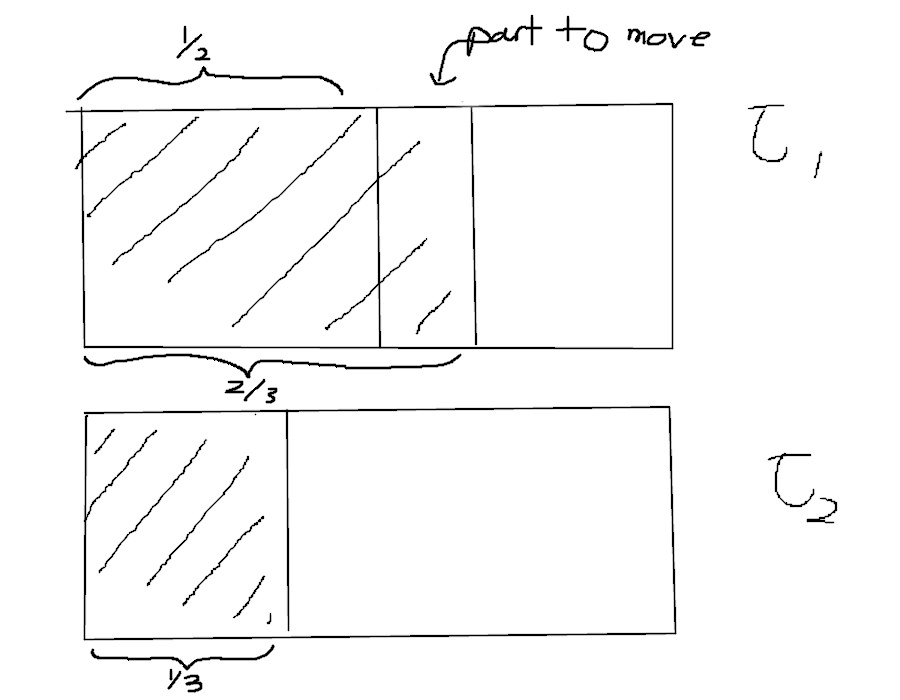
\includegraphics[valign=m,width=250px]{cscc73-a8-q1-diagram1.jpg}
	\end{center}

	For the condition that $T_2 \geq 2T_1$, we can apply the same contradiction proof,
	which results in the same conclusion.

	~\\\hyperlink{toc}{\hypertarget{2.2}{(b)}}\\
	Without loss of generality, suppose $T_1 \geq T_2$\\

$\exists t_i$ in $T_1$ such that $\big|(T_1 - t_i) - (T_2 + t_i)\big| <= |T_1 - T_2|$ for some $i \in \{1,\ \cdots,\ n\}$\\

	Let $t_j$ be the largest number for the above condition. \\
	Then any change after $t_j$ should reduce the absolute difference by less than $t_j$. \\
	If we move $t_j$ again, that implies that we have increased $T_2$ so that $T_2 \geq t_j + T_1$, but this is impossible because
	any element moved from $T_1$ to $T_2$ after $t_j$ must be less than $t_j$. And for the element to have been moved, $T_1 \geq T_2$

	~\\\hyperlink{toc}{\hypertarget{2.3}{(c)}}\\
	Let the job times be $\{5,\ 6,\ 7,\ 8\}$\\
	We can get an arbitrary allocation as follows:\\
$T_1 = \{5,\ 6\}$\\
$T_2 = \{7,\ 8\}$\\

$\sum\limits_{j\in T_1} t_j = 11$\\
$\sum\limits_{j\in T_2} t_j = 15$\\
	For this heuristic, moving any job here would increase the absolute difference, not reduce.
	So the algorithm would halt here after the arbitrary allocation with no movement of jobs.\\\\

	But the optimal solution is:\\
$T_1 = \{5,\ 8\}$\\
$T_2 = \{6,\ 7\}$\\

$\sum\limits_{j\in T_1} t_j = 13$\\
$\sum\limits_{j\in T_2} t_j = 13$\\

	\newpage
	~\\\hyperlink{toc}{\hypertarget{2.4}{(d)}}\\
	Let $N = 2 \times \sum\limits_{i = 1}^{n}t_i$\\

	Objective function:\\
	% $\min \left|\sum\limits_{i=1}^{n} (t_i \times z_i) - \big(t_i \times (1 - z_i)\big) \right|$\\
$\min Z$\\

	Constraints:
	$$
		\begin{array}{r@{}>{\displaystyle}ll}
			z_i                                                                          & {} \in \{0,\ 1\} & \forall i \in \{1,\ 2,\ \ldots\ ,\ n\} \\
			\sum\limits_{i=1}^{n} \big(t_i z_i - t_i (1 - z_i)\big) + N\times Y          & {} \geq Z                                                 \\
			- \sum\limits_{i=1}^{n} \big(t_i z_i - t_i (1 - z_i)\big) + N\times (1 - Y ) & {} \geq Z                                                 \\
			X                                                                            & {} \leq Z                                                 \\
			-X                                                                           & {} \leq Z                                                 \\
			Y                                                                            & {} \in \{0,\ 1\}                                          \\
		\end{array}
	$$

	For each job $t_i$, we have $z_i$ to indicate if it's in the first machine or the second machine. The objective function should be
$\left|\sum\limits_{i=1}^{n} (t_i \times z_i) - \big(t_i \times (1 - z_i)\big)\right|$. However, because this is
	not a linear function, it is instead replaced by the variable $Z$. $Z$ is set to $\sum\limits_{i=1}^{n} \big(t_i z_i - t_i (1 - z_i)\big)$
	or $-\sum\limits_{i=1}^{n} \big(t_i z_i - t_i (1 - z_i)\big)$ based on $Y$.\\

	If $Y = 0$, we get
	$$
		\begin{array}{r@{}>{\displaystyle}ll}
			\sum\limits_{i=1}^{n} \big(t_i z_i - t_i (1 - z_i)\big)       & {} \geq Z \\
			- \sum\limits_{i=1}^{n} \big(t_i z_i - t_i (1 - z_i)\big) + N & {} \geq Z \\
			\sum\limits_{i=1}^{n} \big(t_i z_i - t_i (1 - z_i)\big)       & {} \leq Z \\
			-\sum\limits_{i=1}^{n} \big(t_i z_i - t_i (1 - z_i)\big)      & {} \leq Z \\
		\end{array}
	$$

	And since $N = 2 \times \sum\limits_{i = 1}^{n}t_i$, we get $- \sum\limits_{i=1}^{n} \big(t_i z_i - t_i (1 - z_i)\big) + N \geq \sum\limits_{i=1}^{n} \big(t_i z_i - t_i (1 - z_i)\big)$\\
	So by constraints 1 and 3, $Z = \sum\limits_{i=1}^{n} \big(t_i z_i - t_i (1 - z_i)\big)$

	\newpage
	If $Y = 1$, we get\\
	$$
		\begin{array}{r@{}>{\displaystyle}ll}
			\sum\limits_{i=1}^{n} \big(t_i z_i - t_i (1 - z_i)\big) + N & {} \geq Z \\
			- \sum\limits_{i=1}^{n} \big(t_i z_i - t_i (1 - z_i)\big)   & {} \geq Z \\
			\sum\limits_{i=1}^{n} \big(t_i z_i - t_i (1 - z_i)\big)     & {} \leq Z \\
			-\sum\limits_{i=1}^{n} \big(t_i z_i - t_i (1 - z_i)\big)    & {} \leq Z \\
		\end{array}
	$$

	And since $N = 2 \times \sum\limits_{i = 1}^{n}t_i$, we get $\sum\limits_{i=1}^{n} \big(t_i z_i - t_i (1 - z_i)\big) + N \geq \sum\limits_{i=1}^{n} \big(t_i z_i - t_i (1 - z_i)\big)$\\
	So by constraints 2 and 4, $Z = -\sum\limits_{i=1}^{n} \big(t_i z_i - t_i (1 - z_i)\big)$
\end{document}
